\chapter{Vectorization}\label{chp:vectorization}
Vectorization, raster-to-vector conversion or image tracing is the conversion of raster graphics to vector graphics. To understand the reason for converting from raster to vector we need to look at some of the properties of both storage techniques.

Raster data is structured as an array of grid cells, also referred to as pixels. Each cell in a raster can be addressed by its position in the array, by row and column number. Since each pixel has it's own value, a raster can represent a range of spatial objects. A point can be represented by a single pixel, an arc represented by a sequence of pixels and an area as a collection of continuous pixels. Vector data is structured as a finite straight line segment defined by its endpoints. The location, or coordinates, of the endpoints, are given with respect to a coordinatization of the plane. The vector representation is not discretized in a grid space the same way as a raster but does follow an implicit grid structure as a result of the nature of computer arithmetic. Like the raster, the vector structure can represent multiple spatial structures. A point is given by its coordinates, an arc represented as a sequence of line segments, each consisting of start and end coordinates and an area represented by its boundary consisting of a collection of vectors.

\begin{figure}[H]
	\centering
	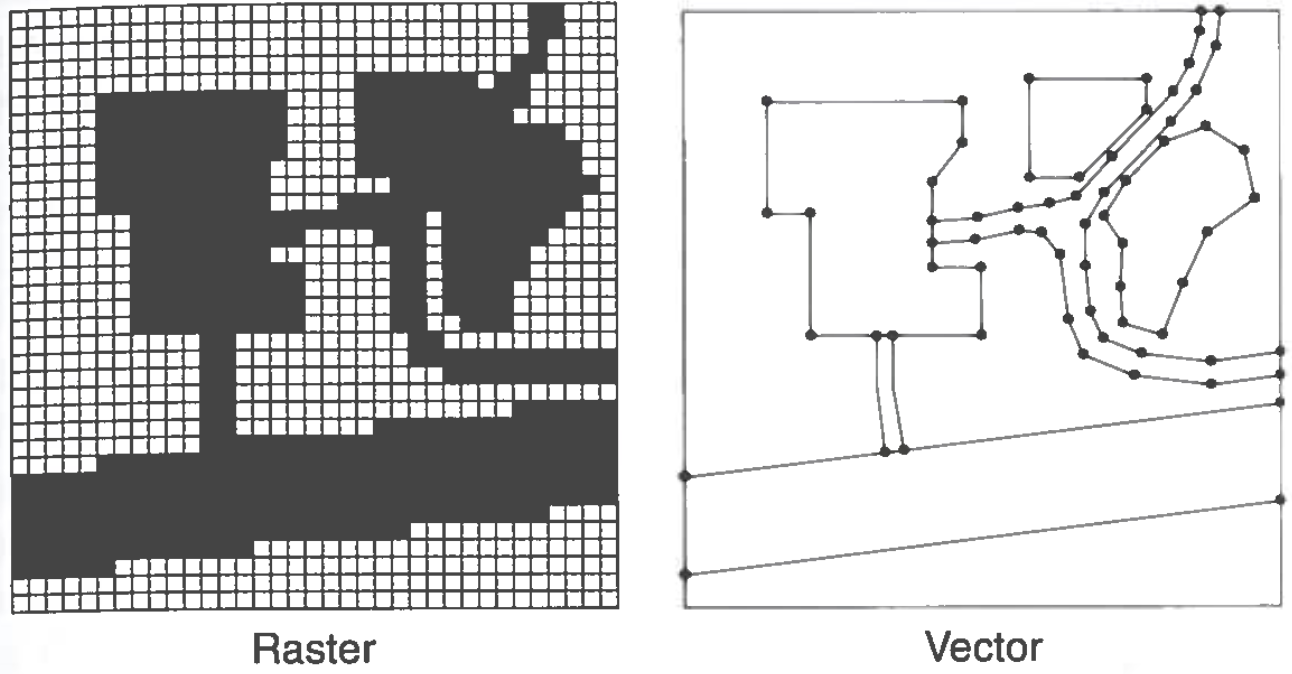
\includegraphics[width=0.8\linewidth]{fig/rastervector.png}
	\caption{Raster and vector data \cite{Worboys2003}}
	\label{fig:rastervsvector}
\end{figure}

There are multiple reasons for storing data in vector format: The geographic accuracy is higher since it is not dependent on grid size. It allows for efficient encoding of topology, an important aspect when doing analysis that utilizes topologic relations, such as proximity and network analysis. Vector data allows for storage of attributes in the data, giving us another dimension of information. The storage size is smaller.

There are multiple different techniques for vectorization. The most known are:

\begin{itemize}
	\item Hough Transform based methods
	\item Thinning based methods
	\item Contour based methods
	\item Run-graph based methods
	\item Mesh pattern based methods
	\item Sparse-pixel based methods
\end{itemize}

All these have different properties and it is important to choose the one that is best for the specific problem. 